\section{Key Telecom Standardization Initiatives} \label{sota:telcoinitiatives}

Section \ref{sota:networkapplications} highlights the importance of telecom standardization initiatives for the definition of network applications and the fulfillment of their use cases. This section provides an overview of the most relevant standards across the industry and academia, outlining the benefits they provide to both developers and operators. In the case of \acs{CAPIF}, this also includes a detailed description of its functional architecture and main entities involved in secure \acs{API} exposure.

\subsection{CAMARA Project} \label{sec:iniatives:CAMARA}

% connection with GSMA not present (should I mention it??)
% INTEROPERABILITY developers, operators, and enterprises

The CAMARA Project, an open-source initiative under the Linux Foundation, focuses on defining, developing and testing simplified telco \acsp{API} to access complex network functions and services. Its primary goals are: (i) simplifying telco complexity through user-friendly \acsp{API} easy to consume for customers with no telco expertise; (ii) facilitating application to network integration; (iii) supporting application portability~\cite{CAMARAProject}.

More specifically, CAMARA abstracts network complexities by presenting a cohesive taxonomy of user-friendly service \acsp{API} throughout a variety of domains, such as network slicing, \ac{QoS} and Location. CAMARA \acsp{API}, being widely adopted by major telecommunication operators and cloud providers (in conjunction with \acs{GSMA}~\cite{CAMARAGSMAindustry}), abstract developers from complex interactions with \ac{5G} Core components, such as the \ac{AMF} and \ac{LMF}, allowing them to integrate advanced network capabilities in a unified ecosystem, while solely focusing on the innovation and design of their own applications.

\hide{\later{Network as a Service -> open and programmable network}}

\subsection{GSMA Open Gateway}

%agilizar - acelerate

The \acs{GSMA} Open Gateway is an initiative lauched by \ac{GSMA} with the goal of establishing a global standardized framework of common network \acsp{API} that simplifies access to mobile operator networks. By giving developers and cloud providers a single point of access to network capabilities provided by multiple operators, \acs{GSMA} Open Gateway promotes simplified integration and service delivery, eliminating the need to individually deal with multiple different operator specific \acsp{API} and accelerating time to market. This is achieved through northbound service \acsp{API}, supported by the CAMARA Project, exposing the mobile operators' network capabilities within a consistent, interoperable and federated framework~\citep{gsmaGSMA,telefonicaGSMA}.

\hide{
6\_Optimizing\_3GPP\_5G\_NEF\_Integration\_Enhancing\_Programmable\_Networks\_Through\_NEF\_and\_UPF\_Interoperability -> abstraction of complexity, introducin CAMARA, CAPIF, reduce time to market 
}

\subsection{CAPIF} \label{sota:initiatives:CAPIF}

% https://www.3gpp.org/technologies/ct3-exp-fr-apis
% https://www.3gpp.org/technologies/rnaa
% https://www.3gpp.org/news-events/3gpp-news/sa6-verticals2

\hide{\later{mention SEAL and NEF support for CAPIF in 5g sba spec (ETSI SPEC)}}


The \acf{CAPIF}, specified by \ac{3GPP}, establishes a single exposure platform for all \ac{3GPP} capability exposure \acsp{API} and non-\ac{3GPP} defined \acsp{API}. The first category includes: (i) Network Northbound \acsp{API} for secure exposure of the \ac{3GPP} core network to external applications via the \ac{SCEF} or \ac{NEF} functions, for \ac{4G} and \ac{5G}, respectively; (ii) Application Enabler Layer \acsp{API} which provide enabler abstraction layers for exposure of common core and application enabler services to external applications. The latter comprises of \acsp{API} defined by other \acs{SDO} or consortiums such as \acs{TMF} or CAMARA~\cite{CapabilityExposure3GPP}. % websites

% Paper CAPIF Microservice & Website
\acs{CAPIF} offers common supporting functionalities applicable to any service \acsp{API} at the northbound of a mobile network. These include on-boarding and off-boarding of \acs{API} invokers, registering and releasing \acsp{API} for exposure and \acs{API} authentication, authorization and discovery by third-parties. This unified framework simplifies and accelerates the delivery of applications (\ac{AF}s) invoking \acsp{API}, while preventing duplication and inconsistences across existing \acs{API} specifications. Furthermore, by allowing third parties to define and publish their own \acsp{API} and securely access 5G core \acsp{API}, CAPIF promotes Network Openness towards Verticals~\cite{CAPIFmicroserviceVerticals}. These capabilites have been fundamental in 3GPP SA6 for facilitating Vertical interaction with the 5G System~\cite{CAPIFSA6}.

% CAPIF ETSI White Paper CAPIF Microservice
% falar dos vários componentes e da arquitetura!!

The \ac{CAPIF} architecture is illustrated in Figure ~\ref{fig:capif-architecture}. It is constituted by three main entities: the \ac{CCF}, the \acs{API} Invoker and the \acs{API} Provider. A brief description of each of the entities and its responsabilities is provided bellow~\citep{CAPIFmicroserviceVerticals,ETSI_CAPIF_TS_123_222_V18_4_0}.

\clearpage


\begin{figure}[htpb]
    \centering
    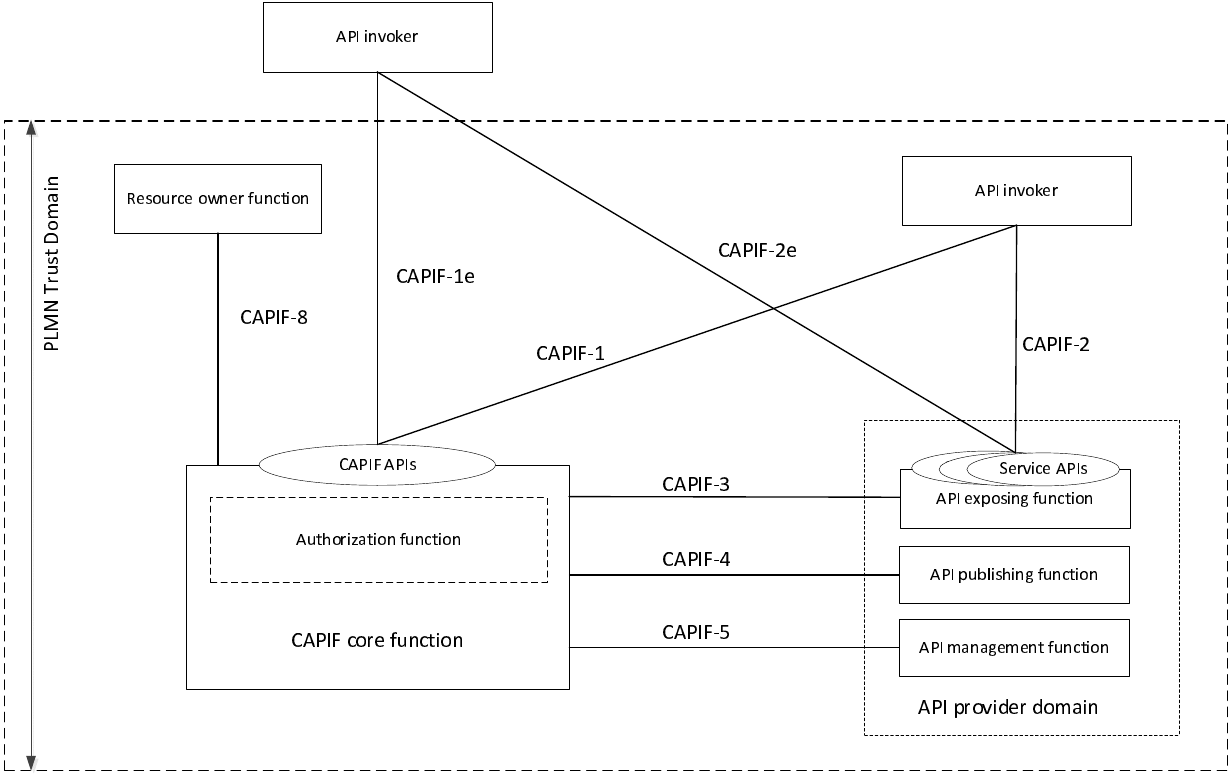
\includegraphics[width=1\linewidth]{figs/capif-architecture.png}
    \caption{High level functional architecture for CAPIF supporting \acs{RNAA}~\cite{ETSI_CAPIF_TS_123_222_V18_4_0}}
    \label{fig:capif-architecture}
\end{figure}


\customparagraph{API Invoker}

The \acs{API} Invoker is typically provided by a third-party application, on a server or \acs{UE}, who has a service agreement with the \acs{PLMN} operator. The \acs{API} Invoker may reside within or outside the \acs{PLMN} operator trust domain and has the following main goal: triggering its onboarding/offboarding and authentication with \acs{CAPIF}, discovering available service \acsp{API} and invoking those \acsp{API} to access network or service capabilities. 

\customparagraph{API Provider}

The \acs{API} Provider represents an entity that owns and exposes \acsp{API} to the \acs{API} Invokers through the CAPIF framework. It provides three different functions: \ac{CAPIFAEF}, \ac{CAPIFAPF} and \ac{CAPIFAMF}.

The \ac{CAPIFAEF} is the service \acs{API} provider and communication entrypoint to the \acs{API} Invokers, handling its authentication and validating the authorization provided by the \ac{CCF} via \acs{JWT}. It is also responsible for logging the service \acs{API} invocations at the \ac{CCF}. The \ac{CAPIFAPF} allows \acs{API} providers to publish their service \acs{API} information to the \ac{CCF} in order to support \acs{API} discovery by \acs{API} invokers. The \ac{CAPIFAMF} lets the \acs{API} provider perform administration of the service \acs{API} including auditing service \acs{API} invocation logs and  monitoring events from \ac{CCF}. It also allows the \acs{API} provider to configure policies to the \ac{CCF}, between other capabilities.

\customparagraph{CAPIF Core Function}

The \ac{CCF} is the core component and acts as the central repository for all published \acsp{API}, controlling service \acs{API} access based on \acs{PLMN} operator configuration policies and handling aspects related to storing (logs provided by the \ac{CAPIFAEF}), auditing, charging and monitoring service \acs{API} invocations. Related to the \acs{API} invoker it is responsible for its onboarding/offboarding, authentication and authorization prior to it accessing the service, as well as publishing, storing and supporting the discovery of service \acs{API} information. In the context of a 4G or 5G system, the \ac{CAPIFAEF} corresponds to the \ac{SCEF} or \ac{NEF} functions.

Lastly, with the goal of \acs{CAPIF} supporting \ac{RNAA} two additional functions are defined: the authorization function and a resource owner function. The former is an internal entity of the \ac{CCF} and interacts with the \ac{CAPIFAEF}, which acts as a resource owner consent enforcement point. The latter interacts with the authorization function via CAPIF-8, which is not specified in the current release of the specification.

\hide{

\later{
\later{TS 33.501}
The security aspects of \acs{CAPIF} supporting RNAA are specified in 3GPP TS 33.122 [12].} \later{The API invoker interacts with authorization function in the CAPIF core function via CAPIF-1/CAPIF-1e.} \later{add diagram and all connections} \later{sequence diagram flow} \later{different authentication mechanisms} \later{add reference to pathway\_towards\_NaaS\_CAMARA.pdf which includes CAPIF}

}


\subsection{TM Forum}
\label{sota:telcoinitiatives:tmf}


\ac{TMF}~\footnote{https://www.tmforum.org/} is a global aliance composed of telco and tech companies from the connectivity ecosystem with the goal of providing a cooperative framework to collaborate and establish industry-wide standards, best practices and toolkits. These include over 800 organizations, encompassing the top 10 \ac{CSP}s, the three leading hyperscalers, major Network Equipment Providers, as well as a diverse array of vendors, consultancies, and system integrators~\cite{aboutTMF}.

The core element of \ac{TMF}'s approach in achieving its missions is the \ac{ODA}. \ac{TMF} \ac{ODA} advocates for the existence of technology agnostic Open \ac{API}s, collaboratively developed by its members to provide standardized interfaces that streamline digital services across a wide range of domains, such as \ac{IoT} or healthcare. In the telecoms industry, the Open \ac{API} Project plays a crucial role in gathering \ac{CSP}s and solution and technology providers to accelerate the deployment of interoperable telecom solutions, tackling integration and delivery complexity while reducing time-to-market~\cite{openAPIsTMF}.

\ac{TMF} Open \ac{API}s rely on a common API data model that is maintained separately from the API specifications: the \ac{TMF} \ac{SID}. This model, used across the Open Digital Architecture and Open APIs, adresses the \ac{CSP}'s need for shared information definitions and models, establishing a standardized way to represent and organize data for implementing business processes. This business model is independent of platform, language or protocol and helps to identify and categorize business entities important to \ac{CSP}s, reducing duplication and promoting consistency and interoperability. More specifically, business entities can be categorized into the following domains: Market \& Sales, Customer, Product, Service, Resource, Business Partner, Enterprise and Common~\cite{SIDTMF}. Three of these domains are essential and widely used across \acfp{OSS}, such as openslice, and are explored further: the Product, Service and Resource domains.

\hide{
\later{mention relation with BSS and OSS} \later{connect with GSMA and CAMARA (i record some of page of their website mentioning it)}
}

\clearpage
\customparagraph{Product}

A Product represents a tangible or intangible item that enterprises such as \ac{SP}s expose and sell to customers for a profit. It is defined in \ac{SID} through a Product Specification detailing its attributes, methods, relationships and constraints, as perceived by the business user and aligned with what the operator intends to sell at a functional level~\cite{SID-MODELS-v250-TMF}.
% maybe other cites

\customparagraph{Service}

A Service represents internally the underlying technical implementation of a Product, which is offered to customers in a commerce perspective. Services can be categorized into \acfp{CFS}, representing, within an organization's infrastructure, the Product the end-customer acquires (e.g. a music streaming service), and \ac{RFS}, which provide the internal implementations required to support a \ac{CFS} in order to deliver its intended functionalities (e.g. recommendation engine supporting music streaming service). Each Service is defined by a corresponding Service Specification~\cite{SID-MODELS-v250-TMF}.

\hide {

\later{mention Service bundles somewhere}
\later{However, the characteristics' values of the instantiated Service will be specific to each instance.}
\later{Service specification can have multiple other service specifications}

}


\customparagraph{Resource}

Resources are the components that support the provision of Services and therefore the delivery of Products to Customers. These include Physical Resources, such as a router or server, and Logical Resources, such as Virtual Machines, \acp{VNF} or software applications, as well as Compound Resources that aggregate them into a single entity. All three Resource types are instantiated from their respective Resource Specifications, as per the specification~\cite{SID-MODELS-v250-TMF}.

